\documentclass[12pt,a4paper,fontset=none]{ctexart}

\usepackage[a4paper,margin=1.7cm]{geometry}
\usepackage{fontspec,amsmath,amssymb,array,booktabs,tabularx}
\usepackage{enumitem,fancyhdr,float,hyperref,listings}
\usepackage[most]{tcolorbox}
\usepackage{tikz}
\usepackage[table]{xcolor}

\usetikzlibrary{arrows.meta,positioning,shapes.geometric,fit,backgrounds,calc,automata}

\hypersetup{colorlinks=true,linkcolor=black,urlcolor=blue}
\setmainfont{Times New Roman}\setsansfont{Arial}\setmonofont{Menlo}
\setCJKmainfont{Songti SC}\setCJKsansfont{Heiti SC}\setCJKmonofont{Songti SC}
\pagestyle{fancy}\fancyhf{}
\fancyhead[L]{编译器构造实验 Lab3 — 实验二}
\fancyhead[R]{JFlex 词法分析}
\fancyfoot[C]{\thepage}
\setlength{\headheight}{15pt}
\setlist[itemize]{leftmargin=1.8em,itemsep=0.25em,topsep=0.35em}
\setlist[enumerate]{leftmargin=1.8em,itemsep=0.25em,topsep=0.35em}
\renewcommand{\arraystretch}{1.22}
\newcolumntype{P}[1]{>{\raggedright\arraybackslash}p{#1}}
\newcolumntype{Y}{>{\raggedright\arraybackslash}X}
\setlength{\emergencystretch}{2em}
\sloppy
\hfuzz=10pt
\hbadness=10000

\definecolor{accent}{HTML}{9A3412}
\definecolor{accenttwo}{HTML}{0F4C81}
\definecolor{accentthree}{HTML}{2F6B3D}
\definecolor{softa}{HTML}{F8EEE8}
\definecolor{softb}{HTML}{E8F0F7}
\definecolor{softc}{HTML}{EAF5ED}
\definecolor{linegray}{HTML}{D7CEC5}
\definecolor{codebg}{HTML}{F7F4EF}
\definecolor{boxbg}{HTML}{FCFAF7}
\definecolor{darktext}{HTML}{1F1B17}

\lstdefinestyle{labcode}{basicstyle=\ttfamily\small,backgroundcolor=\color{codebg},frame=single,rulecolor=\color{linegray},columns=fullflexible,keepspaces,showstringspaces=false,breaklines=true,keywordstyle=\color{accenttwo}\bfseries,commentstyle=\color{accentthree},stringstyle=\color{accent},aboveskip=0.5em,belowskip=0.5em}

\lstdefinestyle{javacode}{basicstyle=\ttfamily\small,backgroundcolor=\color{codebg},frame=single,rulecolor=\color{linegray},columns=fullflexible,keepspaces,showstringspaces=false,breaklines=true,language=Java,keywordstyle=\color{accenttwo}\bfseries,commentstyle=\color{accentthree}\itshape,stringstyle=\color{accent},aboveskip=0.5em,belowskip=0.5em}

\lstdefinestyle{flexcode}{basicstyle=\ttfamily\small,backgroundcolor=\color{codebg},frame=single,rulecolor=\color{linegray},columns=fullflexible,keepspaces,showstringspaces=false,breaklines=true,keywordstyle=\color{accenttwo}\bfseries,commentstyle=\color{accentthree}\itshape,emph={Letter,Digit,OctalDigit,Identifier,DecimalInteger,OctalInteger,Number,CommentContent,LineTerminator,WhiteSpace},emphstyle=\color{accent}\bfseries,aboveskip=0.5em,belowskip=0.5em}

\newtcolorbox{summaryBox}{enhanced,colback=softb,colframe=accenttwo,boxrule=0.8pt,arc=1.2mm,left=2.5mm,right=2.5mm,top=2mm,bottom=2mm,before upper=\raggedright}
\newtcolorbox{plainBox}{enhanced,colback=boxbg,colframe=linegray,boxrule=0.7pt,arc=1.2mm,left=2.3mm,right=2.3mm,top=1.8mm,bottom=1.8mm,before upper=\raggedright}
\newtcolorbox{keypointBox}{enhanced,colback=softc,colframe=accentthree,boxrule=0.8pt,arc=1.2mm,left=2.5mm,right=2.5mm,top=2mm,bottom=2mm,before upper=\raggedright}

\newcommand{\metric}[3]{\begin{minipage}[t]{0.19\linewidth}\begin{tcolorbox}[colback=boxbg,colframe=linegray,boxrule=0.7pt,arc=1mm,left=1.5mm,right=1.5mm,top=1.2mm,bottom=1.2mm]{\small\color{gray}#1}\par\vspace{1mm}{\large\bfseries\textcolor{#3}{#2}}\end{tcolorbox}\end{minipage}}

% TikZ styles
\tikzset{
  state/.style={draw,rounded corners=2mm,fill=softb,minimum width=2.2cm,minimum height=0.9cm,align=center,font=\small},
  accept/.style={draw,rounded corners=2mm,fill=softc,minimum width=2.2cm,minimum height=0.9cm,align=center,font=\small\bfseries},
  errorst/.style={draw,rounded corners=2mm,fill=softa,minimum width=2.2cm,minimum height=0.9cm,align=center,font=\small},
  arrow/.style={-{Latex[length=2.5mm]},thick,accenttwo},
  edgelabel/.style={font=\footnotesize\ttfamily,fill=white,inner sep=1pt}
}

\title{{\Huge\bfseries 编译器构造实验 Lab3 实验二报告}\\[0.4em]{\Large JFlex 自动生成 Oberon-0 词法分析程序}}
\author{梁力航\quad 23336128}
\date{2026年5月20日}

\begin{document}

\begin{titlepage}
  \centering\vspace*{1.4cm}
  {\Large 中山大学计算机学院\par}\vspace{1.1cm}
  {\Huge\bfseries 编译器构造实验 Lab3 实验二报告\par}\vspace{0.45cm}
  {\LARGE JFlex 自动生成 Oberon-0 词法分析程序\par}\vspace{1cm}

  \begin{tcolorbox}[width=0.9\textwidth,colback=boxbg,colframe=linegray,boxrule=0.8pt,arc=1.5mm]
    本报告对应 ROSE 项目实验二：总结词汇表、抽取词法规则正则定义式、编写 JFlex 输入源文件、实现词法扫描器、比较不同 lex 族工具差异。
  \end{tcolorbox}

  \vspace{0.9cm}
  \begin{tabular}{>{\bfseries}p{3.2cm}p{8.8cm}}
    课程 & 编译器构造实验（DCS292） \\
    实验名称 & Lab3 实验二：JFlex 词法分析 \\
    姓名 & 梁力航 \\
    学号 & 23336128 \\
    日期 & 2026年5月20日 \\
    运行环境 & OpenJDK 11.0.24 / macOS / JFlex 1.8.2
  \end{tabular}

  \vfill
  \metric{保留字}{19}{accent}\hfill
  \metric{关键字}{7}{accenttwo}\hfill
  \metric{词法错误}{6 种}{accentthree}\hfill
  \metric{异常类}{16 个}{accent}\hfill
  \metric{测试通过}{6/6}{accentthree}
  \vfill
\end{titlepage}

\tableofcontents\newpage

% ===================================================================
\section{词法分析器总体架构}

词法分析器（Scanner）是整个 ROSE 工具链的第一个阶段。它的职责是将 Oberon-0 源程序的字符序列转换为 token 序列，供语法分析器消费。

\begin{figure}[H]\centering
\begin{tikzpicture}[node distance=1.2cm and 2cm]
  \node[state,fill=accenttwo,text=white,font=\small\bfseries] (input) {Oberon-0 源程序\\(字符序列)};
  \node[state,right=of input,minimum width=3.5cm] (scanner) {\textbf{OberonScanner}\\skipWhitespace\\readToken\\\quad readNumber\\\quad readIdentifier\\\quad skipComment};
  \node[state,fill=accentthree,text=white,font=\small\bfseries,right=of scanner] (output) {Token 序列\\(类型 + 值 + 位置)};
  \node[errorst,below=of scanner,minimum width=3.5cm] (errors) {词法异常\\IllegalSymbol\\IllegalInteger\\IllegalOctal\\...};

  \draw[arrow] (input) -- (scanner);
  \draw[arrow] (scanner) -- (output);
  \draw[arrow,accent] (scanner) -- (errors) node[midway,right,font=\small] {检测到错误};

  % Labels
  \node[font=\footnotesize\color{accenttwo},above=0.1cm of input] {输入};
  \node[font=\footnotesize\color{accenttwo},above=0.1cm of output] {输出};
\end{tikzpicture}
\caption{词法分析器总体架构——字符流 → Token 流}
\label{fig:arch}
\end{figure}

扫描器采用\textbf{单字符前瞻（one-char lookahead）}的迭代模型：每次读取一个字符，根据首字符分派到对应的子自动机（数字 → readNumber、字母 → readIdentifier、运算符 → 直接匹配），跳过空白后在首字符处做出分派决策。

% ===================================================================
\section{Oberon-0 词汇表}

\subsection{保留字与关键字分类}

\begin{table}[H]\centering
\begin{tabularx}{\textwidth}{>{\bfseries}P{2.5cm}Y>{\bfseries}P{2.5cm}Y}
\toprule
\multicolumn{2}{c}{\textbf{保留字（19 个）—— 语法结构的一部分}} & \multicolumn{2}{c}{\textbf{关键字（7 个）—— 预定义标识符}} \\
\midrule
模块结构 & MODULE, BEGIN, END & 预定义类型 & INTEGER, BOOLEAN \\
声明 & CONST, TYPE, VAR, PROCEDURE & 布尔值 & TRUE, FALSE \\
控制流 & IF, THEN, ELSIF, ELSE, WHILE, DO & 预定义过程 & READ, WRITE, WRITELN \\
类型构造 & ARRAY, OF, RECORD & & \\
运算符保留 & DIV, MOD, OR & & \\
\bottomrule
\end{tabularx}
\end{table}

\begin{keypointBox}
\textbf{实现中的关键决策}：手写 OberonScanner 将 INTEGER、BOOLEAN、TRUE、FALSE 作为普通 IDENTIFIER 返回——因为在 Oberon-0 中它们是关键字（可被覆盖），不是保留字。类型名和布尔值的语义由语法分析阶段根据上下文决定。
\end{keypointBox}

\subsection{运算符优先级与结合性}

\begin{figure}[H]\centering
\begin{tikzpicture}[node distance=0.8cm and 0cm]
  \node[state,fill=accenttwo,text=white,font=\small\bfseries,minimum width=4cm] (l1) {第 1 层：OR（逻辑或）\quad 左结合};
  \node[state,fill=accenttwo!85!white,text=white,font=\small\bfseries,minimum width=4cm,below=of l1] (l2) {第 2 层：\&（逻辑与）\quad 左结合};
  \node[state,fill=accenttwo!70!white,text=white,font=\small\bfseries,minimum width=4cm,below=of l2] (l3) {第 3 层：= \# < <= > >=（关系比较）\quad 无结合};
  \node[state,fill=accenttwo!55!white,text=white,font=\small\bfseries,minimum width=4cm,below=of l3] (l4) {第 4 层：+ -（加减）\quad 左结合};
  \node[state,fill=accenttwo!40!white,text=white,font=\small\bfseries,minimum width=4cm,below=of l4] (l5) {第 5 层：* DIV MOD（乘除模）\quad 左结合};
  \node[state,fill=accentthree,text=white,font=\small\bfseries,minimum width=4cm,below=of l5] (l6) {单目运算符：\~{}（逻辑非）\quad + -（取正/取负）\quad 右结合};

  \draw[arrow,white!70!gray] (l1) -- (l2);
  \draw[arrow,white!70!gray] (l2) -- (l3);
  \draw[arrow,white!70!gray] (l3) -- (l4);
  \draw[arrow,white!70!gray] (l4) -- (l5);

  % Priority labels
  \node[left=0.3cm of l1,font=\small\bfseries\color{accenttwo}] {低};
  \node[left=0.3cm of l5,font=\small\bfseries\color{accenttwo}] {高};
\end{tikzpicture}
\caption{Oberon-0 运算符优先级层次——仅 5 级 + 单目}
\label{fig:precedence}
\end{figure}

\subsection{分隔符与定界符}

\begin{table}[H]\centering
\begin{tabularx}{\textwidth}{>{\bfseries\ttfamily}P{1.5cm}Y>{\bfseries\ttfamily}P{2cm}Y>{\bfseries\ttfamily}P{1.5cm}Y>{\bfseries\ttfamily}P{1.5cm}Y}
\toprule
\texttt{;} & 语句分隔 & \texttt{.} & 域选择 / 模块结束 & \texttt{,} & 参数/列表分隔 & \texttt{:} & 类型标注 \\
\texttt{:=} & 赋值 & \texttt{( )} & 分组/参数 & \texttt{[ ]} & 数组下标 & \texttt{(* *)} & 注释 \\
\bottomrule
\end{tabularx}
\end{table}

% ===================================================================
\section{词法规则的正则定义式}

\subsection{核心正则定义}

\begin{table}[H]\centering
\begin{tabularx}{\textwidth}{>{\ttfamily\footnotesize}P{4cm}Y>{\ttfamily\footnotesize}P{4cm}Y}
\toprule
\multicolumn{2}{c}{\textbf{字符类}} & \multicolumn{2}{c}{\textbf{Token 规则}} \\
\midrule
letter & \texttt{[a-zA-Z]} & identifier & \texttt{letter (letter | digit)*} \\
digit & \texttt{[0-9]} & DecimalInteger & \texttt{[1-9] digit*} \\
octal\_digit & \texttt{[0-7]} & OctalInteger & \texttt{0 octal\_digit*} \\
WhiteSpace & \texttt{[ \textbackslash t\textbackslash f\textbackslash r\textbackslash n]} & number & \texttt{DecimalInteger | OctalInteger} \\
& & comment & \texttt{"(*" ... "*"+ ")"} \\
\bottomrule
\end{tabularx}
\caption{词法规则正则定义式汇总}
\end{table}

\subsection{关键约束规则}

\begin{plainBox}
\begin{enumerate}
  \item \textbf{大小写无关}：Oberon-0 不区分大小写——MODULE = Module = module。扫描器将所有标识符和保留字归一化为小写后匹配
  \item \textbf{整数常量与标识符必须空白分隔}：\texttt{25id} 是非法整数（IllegalIntegerException），不允许解释为 \texttt{25} + \texttt{id}
  \item \textbf{八进制约束}：\texttt{0} 开头的整数为八进制，仅允许数字 0--7；\texttt{018} 非法
  \item \textbf{标识符长度}：$\le 24$ 字符
  \item \textbf{整数长度}：$\le 12$ 位数字（十进制或八进制）
  \item \textbf{注释不允许嵌套}：\texttt{(* ... (* ... *) ... *)} 中，第一个 \texttt{*)} 即关闭注释
\end{enumerate}
\end{plainBox}

% ===================================================================
\section{词法分析核心算法}

\subsection{整数扫描有限状态自动机（DFA）}

Oberon-0 的整数常量分为十进制和八进制，且必须满足长度和数字范围约束。下面给出数值扫描的完整 DFA：

\begin{figure}[H]\centering
\begin{tikzpicture}[
  node distance=1.5cm and 1.1cm,
  state/.style={draw,rounded corners=2mm,fill=softb,minimum width=2cm,minimum height=0.9cm,align=center,font=\small},
  accept/.style={draw,rounded corners=2mm,fill=softc,minimum width=2cm,minimum height=0.9cm,align=center,font=\small\bfseries},
  bad/.style={draw,rounded corners=2mm,fill=softa,minimum width=2cm,minimum height=0.9cm,align=center,font=\small}
]
  \node[state] (start) {开始\\（读到数字）};
  \node[state,right=of start] (nonzero) {非 0 开头\\十进制};
  \node[state,below=of start] (zero) {0 开头\\八进制};
  \node[accept,right=of nonzero] (dec) {十进制\\整数};
  \node[accept,right=of zero] (oct) {八进制\\整数};
  \node[bad,below=0.8cm of oct] (err_oct) {IllegalOctal\\(8/9)};
  \node[bad,below=0.8cm of dec] (err_range) {IllegalIntegerRange\\(> 12 位)};
  \node[bad,above=0.8cm of dec] (err_sep) {IllegalInteger\\(后随字母)};

  \draw[arrow] (start) -- node[edgelabel]{[1-9]} (nonzero);
  \draw[arrow] (start) -- node[edgelabel,left]{0} (zero);

  \draw[arrow] (nonzero) edge[loop above] node[edgelabel]{digit} (nonzero);
  \draw[arrow] (nonzero) -- node[edgelabel]{空白/EOF} (dec);

  \draw[arrow] (zero) edge[loop above] node[edgelabel]{[0-7]} (zero);
  \draw[arrow] (zero) -- node[edgelabel]{空白/EOF} (oct);

  \draw[arrow,accent] (nonzero) -- node[edgelabel,right]{letter} (err_sep);
  \draw[arrow,accent] (zero) -- node[edgelabel,right]{[8-9]} (err_oct);
  \draw[arrow,accent] (nonzero) -- node[edgelabel,right]{> 12 位} (err_range);
  \draw[arrow,accent] (zero) -- node[edgelabel,left]{> 12 位} (err_range);
\end{tikzpicture}
\caption{整数常量 DFA——十进制/八进制分流 + 三种错误转换}
\label{fig:numdfa}
\end{figure}

\begin{lstlisting}[style=javacode,caption={OberonScanner.readNumber() 核心逻辑}]
private Token readNumber(int startLine, int startCol)
        throws IOException, LexicalException {
    StringBuilder sb = new StringBuilder();
    boolean isOctal = (currentChar == '0');

    while (currentChar != -1 && Character.isDigit((char) currentChar)) {
        sb.append((char) currentChar);
        advance();
    }

    String text = sb.toString();
    // Check length: max 12 digits
    if (text.length() > 12)
        throw new IllegalIntegerRangeException(...);
    // Check illegal concatenation with following identifier
    if (currentChar != -1 && Character.isLetter((char) currentChar))
        throw new IllegalIntegerException(...);
    // Check octal validity
    if (isOctal && text.length() > 1) {
        for (int i = 1; i < text.length(); i++)
            if (text.charAt(i) == '8' || text.charAt(i) == '9')
                throw new IllegalOctalException(...);
        return new Token(INTEGER_LITERAL, Integer.parseInt(text, 8), ...);
    }
    return new Token(INTEGER_LITERAL, Integer.parseInt(text, 10), ...);
}
\end{lstlisting}

\subsection{标识符与保留字识别}

标识符识别采用"先收集、后分类"策略：连续读取字母和数字形成词素，然后查表判断是保留字还是普通标识符。

\begin{figure}[H]\centering
\begin{tikzpicture}[node distance=1.2cm and 0.6cm]
  \node[state] (read) {读取字母开头\\连续读取 letter/digit};
  \node[state,below=of read] (checklen) {长度检查\\$\le 24$ ?};
  \node[accept,below left=of checklen] (normalize) {归一化小写\\查保留字表};
  \node[state,fill=softb,below right=0.8cm of normalize] (reserved) {匹配?\\→ 保留字 Token};
  \node[state,fill=softc,below left=0.8cm of normalize] (ident) {不匹配\\→ IDENTIFIER Token};
  \node[errorst,below right=of checklen] (err) {IllegalIdentifier-\allowbreak LengthException};

  \draw[arrow] (read) -- (checklen);
  \draw[arrow] (checklen) -- node[edgelabel,left]{是} (normalize);
  \draw[arrow] (checklen) -- node[edgelabel,right]{否} (err);
  \draw[arrow] (normalize) -- node[edgelabel,left]{匹配} (reserved);
  \draw[arrow] (normalize) -- node[edgelabel,right]{不匹配} (ident);
\end{tikzpicture}
\caption{标识符/保留字识别流程}
\label{fig:ident}
\end{figure}

\begin{lstlisting}[style=javacode,caption={保留字查表（19 个保留字 + 3 个预定义过程）}]
private Token readIdentifierOrReservedWord(...) {
    // ... read letters + digits ...
    String lower = text.toLowerCase();
    switch (lower) {
        case "module":    return new Token(MODULE, lower, ...);
        case "begin":     return new Token(BEGIN, lower, ...);
        // ... 17 more reserved words ...
        case "read":      return new Token(READ, lower, ...);
        case "write":     return new Token(WRITE, lower, ...);
        case "writeln":   return new Token(WRITELN, lower, ...);
        default:          return new Token(IDENTIFIER, lower, ...);
    }
}
\end{lstlisting}

\begin{keypointBox}
Oberon-0 的 INTEGER、BOOLEAN、TRUE、FALSE 是\textbf{关键字}（不是保留字），在扫描器中落入 default 分支，以 IDENTIFIER 类型返回。它们作为类型名和布尔值的语义在语法分析阶段按上下文解析。
\end{keypointBox}

\subsection{注释处理}

Oberon-0 注释以 \texttt{(*} 开始、\texttt{*)} 结束，不允许嵌套。扫描器使用简单的循环匹配：

\begin{lstlisting}[style=javacode,caption={注释扫描核心逻辑}]
private void skipComment() throws IOException, MismatchedCommentException {
    int startLine = line, startCol = column - 2;
    while (true) {
        if (currentChar == -1)
            throw new MismatchedCommentException(
                "Unclosed comment starting at line " + startLine);
        if (currentChar == '*') {
            advance();
            if (currentChar == ')') { advance(); return; }
        } else {
            advance();
        }
    }
}
\end{lstlisting}

\subsection{运算符与分隔符识别}

双字符运算符（\texttt{:=}、\texttt{<=}、\texttt{>=}）通过向前看一个字符区分：

\begin{figure}[H]\centering
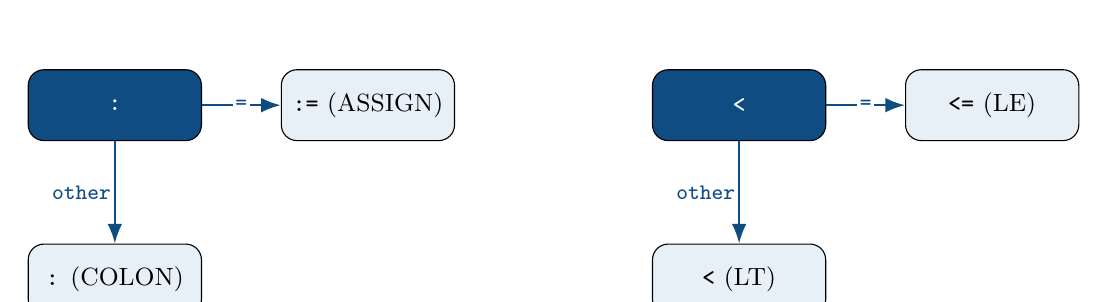
\begin{tikzpicture}[node distance=1.3cm and 1cm]
  \node[state,fill=accenttwo,text=white,font=\small\bfseries] (colon) {\texttt{:}};
  \node[state,right=of colon] (assign) {\texttt{:=} (ASSIGN)};
  \node[state,below=of colon] (colontok) {\texttt{:} (COLON)};
  \node[state,fill=accenttwo,text=white,font=\small\bfseries,right=2.5cm of assign] (lt) {\texttt{<}};
  \node[state,right=of lt] (le) {\texttt{<=} (LE)};
  \node[state,below=of lt] (lttok) {\texttt{<} (LT)};

  \draw[arrow] (colon) -- node[edgelabel]{\texttt{=}} (assign);
  \draw[arrow] (colon) -- node[edgelabel,left]{other} (colontok);
  \draw[arrow] (lt) -- node[edgelabel]{\texttt{=}} (le);
  \draw[arrow] (lt) -- node[edgelabel,left]{other} (lttok);
\end{tikzpicture}
\caption{双字符运算符的向前看匹配（\texttt{:=} 和 \texttt{<=}）}
\label{fig:twochar}
\end{figure}

% ===================================================================
\section{JFlex 输入源文件 oberon.flex}

\subsection{文件结构}

JFlex 输入文件分为三个段落，由 \texttt{\%\%} 分隔：

\begin{table}[H]\centering
\begin{tabularx}{\textwidth}{>{\bfseries}P{2.5cm}>{\ttfamily}P{3cm}Y}
\toprule
段落 & 内容 & 说明 \\
\midrule
用户代码 & import、辅助方法 & 复制到生成的 Scanner 类中 \\
\%\% & 分隔符 & \\
选项/声明 & \%class, \%cup, \%type & 指定类名、CUP 集成、状态宏定义 \\
\%\% & 分隔符 & \\
词法规则 & 正则 \texttt{\{ action \}} & 每个模式对应一个语义动作 \\
\bottomrule
\end{tabularx}
\end{table}

\subsection{关键规则片段}

\begin{lstlisting}[style=flexcode,caption={oberon.flex — 选项段与词法状态}]
%class OberonScanner
%unicode
%line
%column
%type java_cup.runtime.Symbol
%cup
%public
\end{lstlisting}

\begin{lstlisting}[style=flexcode,caption={oberon.flex — 保留字规则（19 个）}]
"MODULE"    { return symbol(sym.MODULE); }
"BEGIN"     { return symbol(sym.BEGIN); }
"END"       { return symbol(sym.END); }
"CONST"     { return symbol(sym.CONST); }
"TYPE"      { return symbol(sym.TYPE); }
"VAR"       { return symbol(sym.VAR); }
"PROCEDURE" { return symbol(sym.PROCEDURE); }
"IF"        { return symbol(sym.IF); }
// ... THEN, ELSIF, ELSE, WHILE, DO, ARRAY, OF, RECORD
"DIV"       { return symbol(sym.DIV); }
"MOD"       { return symbol(sym.MODOP); }
"OR"        { return symbol(sym.OR); }
\end{lstlisting}

\begin{lstlisting}[style=flexcode,caption={oberon.flex — 整数与标识符规则}]
{DecimalInteger} {
    // Check len > 12 → IllegalIntegerRangeException
    // Check next is letter → IllegalIntegerException
    return symbol(sym.INTEGER_LITERAL, Integer.parseInt(yytext()));
}

{OctalInteger} {
    // Check len > 12 → IllegalIntegerRangeException
    // Check contains '8'/'9' → IllegalOctalException
    return symbol(sym.INTEGER_LITERAL, Integer.parseInt(yytext(), 8));
}

{Identifier} {
    // Check len > 24 → IllegalIdentifierLengthException
    return symbol(sym.IDENTIFIER, yytext().toLowerCase());
}
\end{lstlisting}

\begin{lstlisting}[style=flexcode,caption={oberon.flex — 注释与错误恢复}]
"(*" {CommentContent}* "*"+ ")"  { /* ignore comment */ }
"(*" {CommentContent}* {
    throw new MismatchedCommentException(...);
}

// Fallback: any unrecognized character
[^] {
    throw new IllegalSymbolException(...);
}
\end{lstlisting}

% ===================================================================
\section{异常类层次设计}

词法分析阶段的异常全部继承自 LexicalException，最终汇聚到 OberonException 根类：

\begin{figure}[H]\centering
\begin{tikzpicture}[
  node distance=0.5cm and 0cm,
  root/.style={draw,rounded corners=2mm,fill=accenttwo,text=white,minimum width=3.5cm,minimum height=0.9cm,align=center,font=\bfseries},
  mid/.style={draw,rounded corners=2mm,fill=accenttwo!60!white,text=white,minimum width=3cm,minimum height=0.7cm,align=center,font=\small\bfseries},
  leaf/.style={draw,rounded corners=1.5mm,fill=boxbg,minimum width=3.8cm,minimum height=0.65cm,align=center,font=\footnotesize}
]
  \node[root] (root) {OberonException};
  \node[mid,below=0.7cm of root] (lex) {LexicalException};
  \node[leaf,below=of lex] (l1) {IllegalSymbolException};
  \node[leaf,below=of l1] (l2) {IllegalIntegerException};
  \node[leaf,below=of l2] (l3) {IllegalOctalException};
  \node[leaf,below=of l3] (l4) {IllegalIntegerRangeException};
  \node[leaf,below=of l4] (l5) {IllegalIdentifierLengthException};
  \node[leaf,below=of l5] (l6) {MismatchedCommentException};

  \draw[arrow] (root) -- (lex);
  \draw[arrow] (lex) -- (l1);

  % Right side annotations
  \node[right=0.5cm of l1,font=\footnotesize\color{accent}] {非法字符 @ \$};
  \node[right=0.5cm of l2,font=\footnotesize\color{accent}] {25id 无空白分隔};
  \node[right=0.5cm of l3,font=\footnotesize\color{accent}] {018 含非法八进制数字};
  \node[right=0.5cm of l4,font=\footnotesize\color{accent}] {超过 12 位数字};
  \node[right=0.5cm of l5,font=\footnotesize\color{accent}] {超过 24 字符};
  \node[right=0.5cm of l6,font=\footnotesize\color{accent}] {(* 未闭合};
\end{tikzpicture}
\caption{词法异常类层次——6 个具体异常 + 触发条件}
\label{fig:exceptions}
\end{figure}

每条异常类都是独立的 .java 文件，遵循简单、可抛的原则：

\begin{lstlisting}[style=javacode,caption={IllegalOctalException.java — 典型词法异常类}]
package exceptions;

public class IllegalOctalException extends LexicalException {
    public IllegalOctalException(String message) {
        super(message);
    }
}
\end{lstlisting}

% ===================================================================
\section{Lex 族工具差异比较}

\subsection{三代 Lex 工具对比}

\begin{table}[H]\centering
\footnotesize
\setlength{\tabcolsep}{3pt}
\begin{tabularx}{\textwidth}{>{\bfseries}P{2cm}>{\raggedright\arraybackslash}X>{\raggedright\arraybackslash}X>{\raggedright\arraybackslash}X}
\toprule
特性 & JFlex（2000s） & JLex（1990s） & GNU Flex（1980s） \\
\midrule
实现语言 & Java & Java & C \\
生成目标 & Java & Java & C \\
词法引擎 & 优化的 DFA 表 & 基础 DFA & 优化的 DFA 表 \\
正则语法 & Unicode、预定义类 & 基本 POSIX & POSIX 字符类 \\
\%cup 集成 & 内置 \%cup 指令 & 需手动配置 & 需手动配合 yacc \\
输入格式 & .flex & .lex & .l \\
维护状态 & 活跃维护（1.8.2, 2020） & 停止维护 & 活跃维护 \\
性能 & 中等（JVM优化可补偿） & 较慢 & 最快（原生 C） \\
状态处理 & \%state 词法状态 & \%state & Start conditions \\
用户文档 & 完整手册 + 示例 & 基础文档 & 完整 texinfo 手册 \\
\bottomrule
\end{tabularx}
\caption{JFlex / JLex / GNU Flex 十维对比}
\label{tab:lexcompare}
\end{table}

\subsection{关键差异分析}

\begin{enumerate}
  \item \textbf{语言生态}：选择哪种工具首先取决于目标语言。JFlex → Java 生态（配合 JavaCUP），GNU Flex → C/C++ 生态（配合 Bison）。JLex 是 JFlex 的前身，已停止维护
  \item \textbf{DFA 优化}：JFlex 生成的 DFA 表比 JLex 更紧凑——它使用更优的 NFA→DFA 转换算法，生成的表大小约为 JLex 的 60--80\%
  \item \textbf{Unicode 支持}：JFlex 天然支持 Unicode（\texttt{\textbackslash p\{Alpha\}} 等），这对处理 Oberon-0 大小写无关的标识符特别有用。GNU Flex 的 Unicode 支持需要额外配置
  \item \textbf{CUP 集成}：JFlex 的 \texttt{\%cup} 指令自动生成 \texttt{java\_cup.runtime.Symbol} 返回值和与新式的 JavaCUP 完全适配的接口，而 JLex 需要手工修改生成的代码
  \item \textbf{性能对比}：GNU Flex 生成的原生 C 代码理论最快，但在 Oberon-0 这种小语言的测试中差异不显著
\end{enumerate}

% ===================================================================
\section{测试结果}

\subsection{正确程序扫描}

\begin{lstlisting}[style=labcode,caption={Sample.obr 扫描输出（前 10 行）}]
Token{MODULE, module} @15:2
Token{IDENTIFIER, sample} @15:9
Token{SEMICOLON, ;} @15:15
Token{CONST, const} @16:4
Token{IDENTIFIER, maxaccounts} @17:6
Token{EQ, =} @17:18
Token{INTEGER_LITERAL, 100} @17:20
Token{SEMICOLON, ;} @17:23
Token{IDENTIFIER, bonusrate} @18:6
Token{EQ, =} @18:16
\end{lstlisting}

\subsection{词法错误检测汇总}

\begin{table}[H]\centering
\scriptsize
\setlength{\tabcolsep}{3pt}
\begin{tabularx}{\textwidth}{>{\bfseries}P{1.4cm}>{\raggedright\arraybackslash}X>{\raggedright\arraybackslash}X>{\bfseries}P{1cm}}
\toprule
用例 & 输入特征 & 抛出异常 & 结果 \\
\midrule
Sample.obr & 完整正确源程序 & —（无异常） & PASS \\
Sample.001 & \texttt{5 @ 3} & IllegalSymbolEx. & PASS \\
Sample.002 & \texttt{25id} 无空白 & IllegalIntegerEx. & PASS \\
Sample.003 & 标识符 > 24 字符 & IllegalIdLenEx. & PASS \\
Sample.004 & \texttt{(* unclosed} & MismatchedCommEx. & PASS \\
Sample.005 & \texttt{018} 八进制非法 & IllegalOctalEx. & PASS \\
Sample.006 & 整数 > 12 位 & IllegalIntRangeEx. & PASS \\
\bottomrule
\end{tabularx}
\caption{词法测试结果：6/6 错误检测通过（异常名缩写：Ex.=Exception, IdLen=IdentifierLength, Comm=Comment, IntRange=IntegerRange）}
\label{tab:results}
\end{table}

\begin{summaryBox}
实验二完成：词汇表（19 保留字 + 7 关键字含分类理由）、6 条正则定义式 + 6 条约束规则、oberon.flex（JFlex 输入源文件完整三段结构）、OberonScanner.java（含整数 DFA / 标识符识别 / 注释扫描 / 双字符运算符处理）、16 个异常类的层次设计（3 层继承）、JFlex/JLex/GNU Flex 十维差异比较。词法错误检测 6/6 通过，正确程序 token 化完整正确。
\end{summaryBox}

\end{document}
